\chapter{Real-Time Scheduling}
\label{chapter.RTS}
This chapter contains a high-level description of the work performed in Samsung Electronics Research Institute UK (SRUK) where I practiced my internship.
This part of work slightly differs of the rest of this thesis as in this chapter we are focused on thread-level scheduling for asymmetric multi-core (AMC) systems.
This means that we are no longer using parallel high-performance applications, rather than mobile phone applications that are implemented in parallel and execute on multiple user-level threads.
Our work focuses on scheduling efficiently those threads among the cores of the system in real-time.
For simplicity, we refer to threads as tasks.

This work presents a showcase for a real-time CPU scheduler with the goal to increase the frames per second (FPS) during the gameplay on mobile devices with the ARM big.LITTLE architecture. 
We design and implement the scheduler in the Android framework and provide an efficient scheduling policy that takes into account the current temperature and performs task migration. 
Our solution increases the median FPS of the currently used mechanisms by up to 7.5\% and at the same time it maintains temperature stable. 
\newpage

\section{Background and Motivation}
It has become common for current mobile devices to use asymmetric mobile processors. 
The state-of-the-art leading asymmetric processor architecture is the ARM big.LITTLE architecture~\cite{Greenhalgh2011} that combines fast out-of-order big cores with simple in-order little cores in order to achieve high performance in a low power budget. 
Even though AMC systems are being used in the mobile market since the early 2013 there is still a lot of work to be done in order to efficiently utilize them.

As we saw in Chapter~\ref{chapter.study} the current thread scheduling techniques take place in the Linux kernel.
The state of the art Linux scheduler “Completely Fair Scheduler” (CFS) \kc{add reference!} manages to be fair by allowing tasks to execute for the same amount of time on each processor. 
CFS maintains load balance among the cores of the system by providing equal portions of processor time to the running tasks. 
Taking into account the asymmetry of current mobile processors and the different types of running applications we can see that CFS contradicts to the needs of an asymmetric system.
This is because a fair distribution of the tasks on an AMC system leads to load imbalance and wrong scheduling decisions. 
Surprisingly enough, CFS is the main scheduler currently used in the mobile market.
Heterogeneous Multi-Processing (HMP) with Global Task Scheduling (GTS) (described in Section\ref{sec:scheduling}) is an enhancement in CFS towards the efficient scheduling of the AMC system. 

Even though HMP solutions take into account the system's asymmetry they fall short on achieving efficient schedules.
The main reason that these attempts fail is that in the kernel level there is not enough information for the scheduler in order to take efficient scheduling decisions.
Information such as data dependencies, task criticality or whether a task is memory or computational bound is not available at kernel level.


%%should take place in the runtime system level.
%From our profiling and evaluation of this existing scheduler, we saw that most of the times, critical threads of the game are scheduled on little cores of the system, causing a drop to the FPS, which makes the user less satisfied. 
%This was our initial motivation for proceeding in the direction of implementing a scheduling solution that takes into account the importance of some threads as well as the asymmetry of the system.
%
%
%
%Scheduling of tasks on such architectures becomes more challenging as an efficient scheduler has to take into account the asymmetry of the system in order to maintain load balance. 
%The state of the art Linux scheduler named “Completely Fair Scheduler” (CFS) manages to be fair by allowing tasks to execute for the same amount of time on each processor. 
%This contradicts to the needs of an asymmetric system as a fair distribution of the tasks on an asymmetric system would lead to load imbalance and wrong scheduling decisions. 
%Heterogeneous Multi-Processing (HMP) is an enhancement in CFS towards the solution of this challenge. 
%However, our primary investigation on games showed that even by using HMP in CFS, the system is not always taking the right decisions for task migration. 
%From our profiling and evaluation of this existing scheduler, we saw that most of the times, critical threads of the game are scheduled on little cores of the system, causing a drop to the FPS, which makes the user less satisfied. 
%This was our initial motivation for proceeding in the direction of implementing a scheduling solution that takes into account the importance of some threads as well as the asymmetry of the system.




%The goal of this internship was to improve game performance (frames per second, FPS) through scheduling of tasks on mobile devices.
Game performance is one of the most challenging areas for mobile devices.
Games are the most demanding mobile applications as they execute very computationally intensive tasks in order to produce the graphics that have to be drawn on the screen.
State-of-the-art mobile games are typically multi-threaded using existing frameworks and run on both CPU and GPU of the system.
Even though the graphics quality and on-screen representation are mainly taking place in the GPU, there are very important CPU tasks that drive the entire game playing procedure.
The CPU tasks are responsible for performing the logic of the game as well as sending the appropriate data (that usually are outputs of the game functions) to the GPU.
One example of these tasks is the Render task that is responsible for writing the appropriate data in a buffer which is then to be read by the GPU kernels that draw the frames on the screen of the device.
Such tasks have to be executed at a specific rate because if they do not finish on time the frame drawing is delayed and then the frame is missed, resulting to screen freezing or FPS drop.
Our solution performs CPU scheduling to increase FPS in games while keeping temperature stable.

%To approach this challenge we had to break the problem into several steps. 
%Below we briefly describe the steps taken:
%1.	Profiling and evaluation of the baseline: at this step we conducted a study to explore the current performance and limitations of the device while running games. An initial evaluation proved that there is room of improvement of frame rate by modifying the scheduling as well as other parameters of the governor.
%2.	Design process: in this step we explored the possibilities of implementing a scheduler. This step was the pathway to the implementation of a final solution as it led us to choose the appropriate programming framework to implement a scheduling solution. This was based on the programming flexibility as well as on the available tools and resources.
%3.	Implementation and experimentation: In this step, after the design and software core implementation was done, we experimented with different policies and tuned the scheduler until we reached the desired result.
%4.	Evaluation: In this step we evaluated our solution on several different games. We compared our solution against the baseline as well as against other mainstream scheduling solutions that we implemented and we got satisfactory results.

\section{Real-Time Scheduling Solution}

%During the design process we experimented with different levels of the software stack for finding the most appropriate level for such an implementation. 
\footnote{This section intentionally lacks detailed description due to NDA agreement with Samsung}As mentioned above, as well as in Chapter~\ref{chapter.study}, scheduling in the kernel level is not flexible and usually results to bad scheduling decisions.
%requires a lot of time and is not flexible. 
An important drawback of the kernel level scheduling is that information provided at this level is limited. 
For example there is no way to know what each task is used for and what the current runtime circumstances are. 
To avoid these obstacles, we move upwards in the software hierarchy and create the appropriate environment to reuse existing Samsung software within the Android framework in order to apply scheduling solutions. 
The Samsung’s Temperature Control (STC) is a system service of the Android framework used to maintain device temperature, that starts execution whenever it detects that a game application is running.
We implement the Real-Time Scheduler (RTS) within STC.
%We implement our solution within a system service of the Android framework that starts execution whenever it detects that a game application is running.

Since temperature plays a very important role in the performance of the mobile device, RTS uses this information in order to make scheduling decisions for the tasks of the executing game.
The scheduling decisions of RTS depend mostly on temperature; RTS decides the appropriate task migration cluster and it then performs the scheduling.
During the game-play, when RTS detects that the temperature increases, it gradually starts migrating tasks of the game to the little-core cluster of the AMC.
In the opposite scenario, when temperature is decreasing, RTS manages to migrate tasks that currently run on the little-core cluster, back to the big-core cluster.
RTS scheduling mechanisms are able to maintain load balance among the cores of the AMC system resulting to higher FPS.

%To find the appropriate scheduling policy
%This would include the data and runtime circumstances that the scheduler should use to make scheduling decisions. 
%From this step we found that temperature plays a very important role in FPS performance. 
%Thus we used this information to make scheduling decisions for the tasks of the executing game. 
%When our scheduler detects that the temperature increases, it gradually starts migrating tasks of the game to the little cluster.
%In the opposite scenario, when temperature is decreasing the scheduler manages to migrate tasks that run on the little cluster, back to the big cluster.
%Finding the correct balance between temperature and task migration required a lot of experimentation and profiling of our solution.

\section{Evaluation}
\subsection{Methodology}
\label{sec.rts.methodology}
We evaluate RTS by using it while running commodity mobile games on a state-of-the-art Samsung mobile device featuring a Samsung Exynos octa-core chip-set with Arm big.LITTLE architecture~\cite{samsung,Greenhalgh2011}. 
We run three mobile games:
\textit{i)} Lineage2~\cite{Lineage}, \textit{ii)} King of Glory~\cite{KOG} and \textit{iii)} Dynasty Warriors~\cite{Dynasty}.
The selected games are battle play games and they all fulfill the criteria that facilitate the evaluation: \textit{(a):} They all have high FPS up to 60 and demanding graphics, \textit{(b):} they have auto-play mode and \textit{(c):} their automatic game-play occurs without intervals for a long time.
Our experiments compare our approach (STC + RTS) against two additional scheduling scenarios:
\begin{itemize}
	\item \textit{GTS:} The default Linux CFS scheduler with the GTS support for asymmetric systems
	\item \textit{STC:} The CFS scheduler with the STC framework enabled during the game-play
	\item \textit{STC + RTS:} The RTS running on top of the STC framework
\end{itemize}
%	We conduct experiments using RTS on top of the STC framework. 
%	We compare our results to the default version of STC and to the default version without using STC. 
Our experiments include 10 runs for each game-scheduler pair and each run lasts for 800 seconds. 
The reported results include the averages among the 10 runs of the median Frames per Second (FPS), the average Prescribed Surface Temperature (PST) and the FPS stability.
The FPS stability characterizes how stable is the FPS during the gameplay. 
We compute the stability by computing the percentage of FPS readings that are at maximum 20\% above or below the median FPS.
%
%
%The final step of our activities was to evaluate our approach. 
%We used three different games: Lineage2, King of Glory and Dynasty Warriors. The specific games were selected because they fulfilled the following criteria:
%1.	High FPS up to 60 and demanding graphics
%2.	Auto-play mode
%3.	Playing with no intervals for a long time
%We conducted experiments using our policy on top of Samsung’s Temperature Control (STC) framework used to maintain the temperature to the desired levels. 
%We compare our results to the default version of STC and to the default version without using STC. 
%Our experiments include 10 runs for each game-scheduler pair and each run takes up to 800 seconds. 
%The reported results show the average among the 10 runs.

\subsection{Results}
\subsubsection{Impact of RTS}
\begin{figure}[t]%
	\centering
	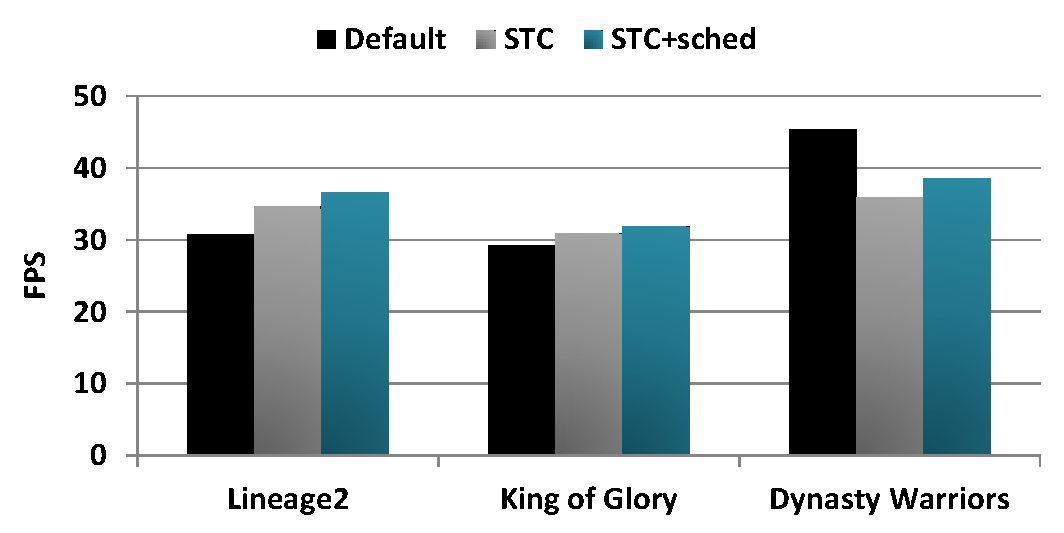
\includegraphics[width=0.7\textwidth]{figures/FPS.pdf}
	\caption{Median frames per second (FPS) results for each game (x axis) and scheduling set-up (series).}
	\label{fig:FPS}
\end{figure}

\begin{figure}[h]%
	\centering
	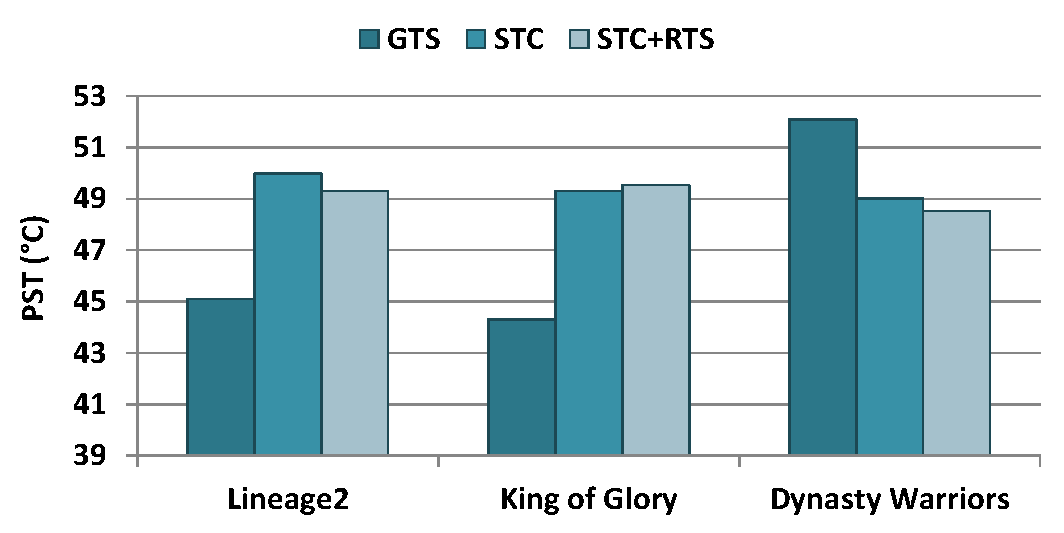
\includegraphics[width=0.7\textwidth]{figures/PST.pdf}
	\caption{Prescribed surface temperature (PST) results for each game (x axis) and scheduling set-up (series).}
	\label{fig:PST}
\end{figure}

Figure~\ref{fig:FPS} shows the median FPS obtained from three games when running on the eight cores of the system using the three different scenarios described above. 
STC+RTS approach improves Samsung's STC by 6\% for Lineage2, by 3\% for King of Glory and by 7.5\% for Dynasty Warriors. 
Figure~\ref{fig:PST} shows the average Prescribed Surface Temperature (PST) observed during the experiments for each game-scheduler.
STC and STC+RTS approaches show similar PST as they both use the same mechanism for the temperature maintenance.
It is important to note that via task scheduling, STC+RTS achieves higher FPS than STC while keeping the temperature at the desired levels, avoiding potential lags due to overheating.

For Dynasty Warriors the GTS approach, that lacks the temperature control, outperforms the approaches that control temperature as shown in Figure~\ref{fig:FPS}. 
This is because in the case of GTS, the default Linux governor and scheduler constantly push the system to achieve higher FPS which potentially leads to device overheating. 
This is verified by the results of Figure~\ref{fig:PST}: the GTS approach maintains the temperature in reasonable levels for Lineage2 and King of Glory, but in the case of Dynasty Warriors the temperature is increased.

%This leads to increased temperature of the device as shown in Figure~\ref{fig:PST}. 
%With this approach, when the temperature increases to a critical point, the device crashes as it has to shut down due to very high temperature.
\begin{figure}[t]%
	\centering
	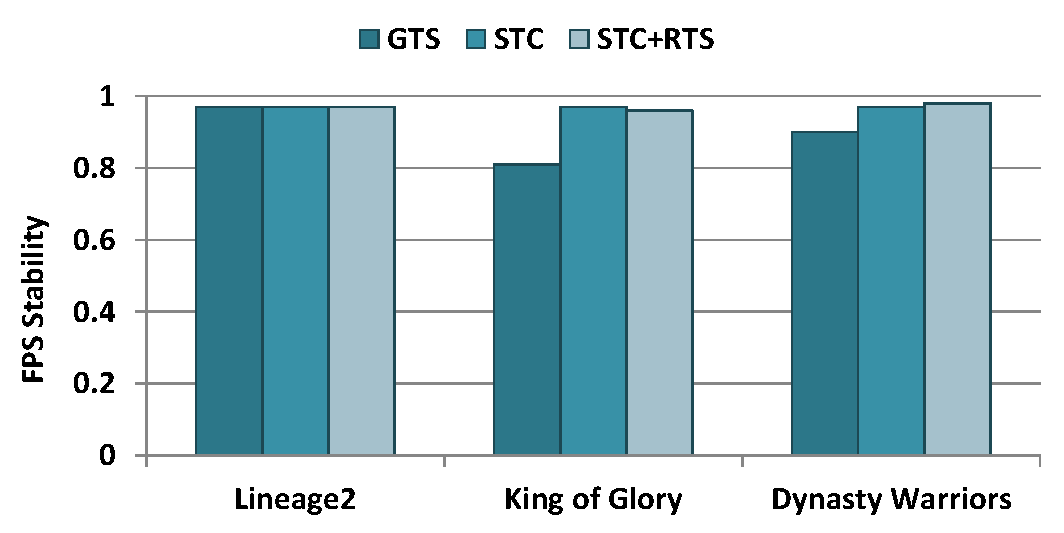
\includegraphics[width=0.7\textwidth]{figures/stability.pdf}
	\caption{FPS stability observed for each game (x axis) and scheduling set-up (series).}
	\label{fig:stability}
\end{figure}

Another important characteristic of the gameplay experience is the FPS stability.
Figure~\ref{fig:stability} shows that FPS stability is not affected by the task scheduling performed with RTS even if tasks migrate from one CPU cluster to another.

\subsubsection{Comparison to Other Approaches}
\begin{figure}[t]%
	\centering
	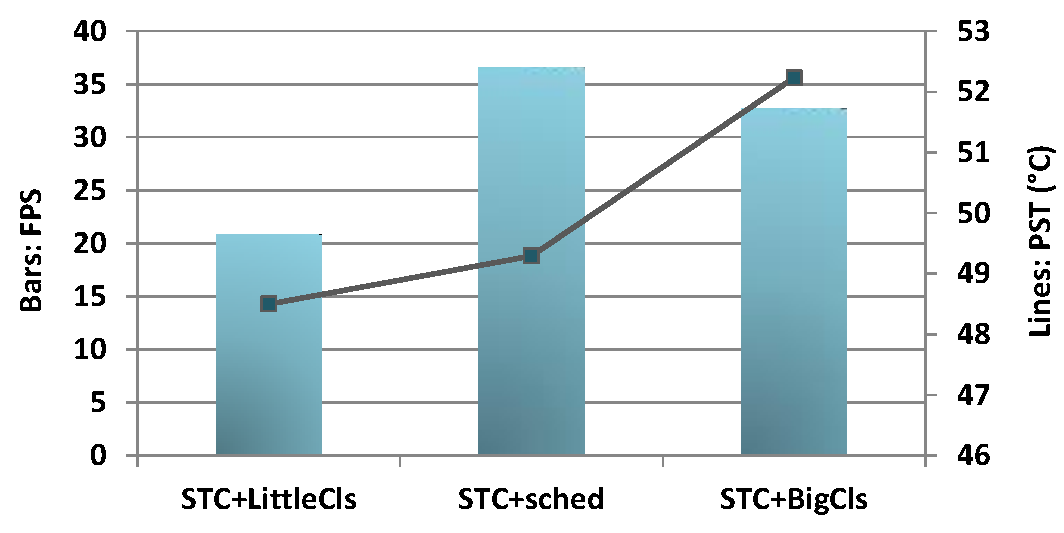
\includegraphics[width=0.7\textwidth]{figures/intern_comparison.pdf}
	\caption{Comparison of the FPS-PST trade-offs for different scheduling policies running on top of STC.}
	\label{fig:int_comparison}
\end{figure}
In this part of the evaluation we compare RTS against two different scheduling approaches that do not involve any sophisticated task migration.
We implement these schedulers on top of STC and we use them to prove that RTS scheduling is effective due to its correct runtime decisions.
The schedulers that we compare in this section are all running together with STC and are the following:
\begin{itemize}
	\item \textit{LittleCls}: in this approach all the tasks of the game are constantly maintained in the little-core cluster
	\item \textit{RTS}: the presented approach, which migrates a number of tasks to the appropriate core cluster according to current temperature
	\item \textit{BigCls:} in this approach all the tasks of the game are constantly maintained in the big-core cluster
\end{itemize} 

Figure~\ref{fig:int_comparison} shows the FPS and temperature results for the aforementioned scheduling approaches when running Lineage2.
The experimental set-up is the same as described in section~\ref{sec.rts.methodology}. 
Maintaining the tasks on the little cluster with LittleCls, significantly limits FPS as the little cores are not as powerful to efficiently process demanding game tasks.
Due to the lack of the big-core cluster use, device temperature is also maintained to very low levels at 48 Celsius degrees.
On the other hand, using only the big-core cluster leads to higher FPS but also increased temperature, even if STC is still operating.
RTS is able to maintain temperature at reasonable levels while achieving the highest FPS due to its efficient scheduling.
It is interesting to note here that running tasks exclusively on the big cluster is not as efficient in terms of FPS.
The increased temperature can affect the governor decisions so the processing power of big cores is reduced leading to FPS decrease as shown in the case of BigCls.


%This figure is used to prove that our solution is effective due to the runtime decisions taken according to the current temperature and runtime circumstances.

\section{Conclusions}

In this chapter we showed that there is significant potential in increasing game performance on mobile devices through task scheduling.
Choosing the right policy is essential as maintaining the tasks to only one core cluster showed its inefficiency.
To maintain load balance on asymmetric systems it is important to decouple the scheduling from the operating system as the Android framework offers more programming flexibility as well as the appropriate runtime information that can be used for the scheduling decisions.
Due to the lack of runtime information, GTS either keeps FPS high at the cost of increased temperature or maintains the temperature low at the cost of lower FPS.
STC+RTS provide a good trade-off between high FPS and reasonable temperature, improving the STC solution. 

